% !TeX program = pdflatex
% Manuscript OUTLINE (annotated skeleton) -- Elsevier / elsarticle format.
% Compile: pdflatex outline.tex (run twice). Images: ../docs/evidence/
\documentclass[preprint,12pt]{elsarticle}

\usepackage[T1]{fontenc}
\usepackage[utf8]{inputenc}
\usepackage{amsmath,amssymb}
\usepackage{booktabs}
\usepackage{tabularx}
\usepackage{graphicx}
\usepackage{subcaption}
\usepackage[colorlinks=true,linkcolor=blue,citecolor=blue,urlcolor=blue]{hyperref}
\graphicspath{{../docs/evidence/}}

\newcommand{\Neq}{N_{\mathrm{eq}}}
\newcommand{\eE}{e_{E}}
\newcommand{\todo}[1]{\textcolor{red}{[#1]}}
\usepackage{xcolor}

% Outline-specific compact list
\newenvironment{plan}{\begin{itemize}\setlength\itemsep{0.15em}}{\end{itemize}}

\journal{Advances in Engineering Software (primary target; alternates listed inside)}

\begin{document}

\begin{frontmatter}

\title{Vision-seeded geodesic partitions with budget-certified region sizing:
adaptive mesh refinement in few solves for three-dimensional bridge components\\
\vspace{0.5em}\normalsize --- MANUSCRIPT OUTLINE v0.1 (2026-08-28, tied to branch
\texttt{cursor/vision-region-amr-gmsh-e89b}) ---}

\author[a]{Author~1\corref{cor}}
\ead{author1@example.org}
\author[a]{Author~2}
\cortext[cor]{Corresponding author.}
\address[a]{Affiliation placeholder, City, Country}

\begin{abstract}
\textbf{[Draft v0; every number below is from the repository pilot runs and must be
regenerated by the full pre-registered campaign before submission.]}
Classical adaptive finite element loops (solve--estimate--mark--refine) are
asymptotically optimal but need many global solves, which is precisely why they are
rarely used on three-dimensional structural components. Practising engineers instead
read the drawing and a coarse stress plot, circle a handful of critical zones, assign
one mesh size per zone, and finalise the mesh within one or two remeshing rounds. We
formalise this workflow: a vision head places \emph{named seeds} on orthographic views
of a probe solution; seeds grow into human-like, geometry-conforming regions as
multi-source geodesic Voronoi cells on the element adjacency graph; each region carries
a single target size, revised by one round of multi-agent negotiation driven by
\emph{measured} regional convergence exponents, and certified by a low-dimensional
particle-swarm calibration that treats the equation budget as a hard cap (closed-form
budget projection, tighten-only resource-drift feedback, late-round trust region,
in-place certification, best-compliant-iterate delivery). All meshes are generated by
Gmsh from nodal size fields; all solves use CalculiX. On two 3D bridge component
families---a bearing block under eccentric patch bearing and a deck panel under
wheel-patch loading---the method reaches lower energy error than a faithfully deployed
element-wise Zienkiewicz--Zhu + D\"orfler loop at equal solve counts $k=2$--$4$
(e.g.\ bearing block: 0.198 vs 0.291 at $k=3$), delivering budget-compliant meshes at
83--94\% of the cap without any offline training; the classical loop overtakes only
from $k^*\!\approx\!5$ solves onward while exceeding the budget. We state this
crossover explicitly and cede asymptotic optimality to D\"orfler by construction.
\end{abstract}

\begin{keyword}
adaptive mesh refinement \sep region-based mesh sizing \sep vision--language models
\sep multi-agent negotiation \sep particle swarm optimization \sep bridge components
\end{keyword}

\end{frontmatter}

% =====================================================================
\section*{Highlights (draft; Elsevier limit: 3--5 bullets, $\le$85 characters each)}
\begin{plan}
  \item Vision-seeded geodesic partitions replace element-wise marking in adaptive FEM.
  \item One negotiation round plus PSO certifies accuracy under a hard equation budget.
  \item Beats D\"orfler at 2--4 solves on 3D bridge bearing and deck panel benchmarks.
  \item Delivered meshes use 83--94\% of the budget cap; overshoot is structurally barred.
  \item Training-free; matches learned baselines that need hundreds of offline solves.
\end{plan}

\section*{Submission package checklist (Elsevier)}
\begin{plan}
  \item Manuscript PDF/source (elsarticle, \verb|preprint| option for initial submission).
  \item Highlights file (above); Graphical abstract: pipeline schematic (Fig.~1 crop,
        $\ge$531$\times$1328 px per spec).
  \item Title page with authors/ORCID; CRediT statement (\S\ref{sec:credit});
        Declaration of competing interests; Data availability statement
        (\S\ref{sec:data}); Funding statement.
  \item Referee suggestions: AMR + ML-for-meshing communities (to be listed).
\end{plan}

\section*{Target venue and article type}\label{sec:venue}
\begin{plan}
  \item \textbf{Primary:} \emph{Advances in Engineering Software} (full-length research
        paper). Fit: engineering workflow formalisation + open-source pipeline; the
        journal published MeshingNet3D~\cite{meshingnet3d}, a direct baseline relative.
  \item \textbf{Alternates:} \emph{Computers \& Structures} (structural FE workflow);
        \emph{Engineering Applications of Artificial Intelligence} (agents/LLM angle);
        \emph{Computer Methods in Applied Mechanics and Engineering} (only if the method
        section is strengthened with a formal analysis of the certified projection);
        \emph{Automation in Construction} (bridge-engineering angle).
  \item Estimated length: 30--35 manuscript pages, 8 figures, 6 tables, 2 appendices.
\end{plan}

% =====================================================================
\section{Introduction}\label{sec:intro}
\textbf{Purpose: establish the narrow claim --- ``fewest global solves to an
engineering-grade mesh under a hard resource cap'', not asymptotic optimality.}
\begin{plan}
  \item Cost model: on 3D solid components each AMR cycle costs one global solve;
        8--12 cycles is exactly why practitioners avoid adaptive FEM
        (\S1.1 of the experiment plan).
  \item The human protocol: read drawing + coarse contour plot $\rightarrow$ circle a
        few zones $\rightarrow$ one size per zone $\rightarrow$ finalise in 1--2
        remeshes. This paper is its formalisation and quantitative defence.
  \item Problem statement (informal): given instance, equation budget $\Neq^{\max}$ and
        solve budget $k_{\max}$, deliver a budget-compliant mesh minimising energy
        error, counting \emph{every} global solve including the probe.
  \item Pre-registered hypotheses H1--H4 (verbatim from the plan, \S\ref{sec:disc}):
        few-solve superiority; hard-cap compliance [90\%,105\%]; training-free parity;
        honest crossover $k^*$.
  \item Contributions:
  \begin{plan}
    \item[C1] Human-like partition representation: named vision seeds grown into
          geodesic Voronoi regions on the element adjacency graph; residual-driven
          region splitting; \emph{regions are never boxes}.
    \item[C2] Budget-certified few-solve loop: one communication round with measured
          exponents + $(s,\kappa)$ PSO under a hard cap with closed-form projection,
          tighten-only drift feedback, trust region, in-place certification and
          best-compliant-iterate delivery semantics.
    \item[C3] Faithful single-mesher redeployment of four comparison methods
          (D\"orfler, one-step local prediction, region-graph DQN, supervised size
          field) with pre-registered axes and machine-checkable validity gates G1--G7.
    \item[C4] Evidence on 3D bridge components that the loop wins at $k=2$--$4$ while
          explicitly exhibiting the crossover where element-wise marking prevails.
  \end{plan}
  \item Scope disclaimer paragraph: linear elasticity, C3D4, ZZ indicator; the claim is
        about \emph{solve-count efficiency under a cap}, nothing else.
\end{plan}

\section{Related work}\label{sec:related}
\textbf{Purpose: four clusters, one gap.} (Table~\ref{tab:related}; representative
citations to be completed.)
\begin{table}[h]\centering\small
\caption{Related-work map (manuscript Table 1).}\label{tab:related}
\begin{tabularx}{\textwidth}{lXX}
\toprule
Cluster & Representatives & Relation to this paper \\
\midrule
Classical element-wise AFEM & D\"orfler~\cite{dorfler96}; ZZ~\cite{zz87};
  Babu\v{s}ka--Rheinboldt~\cite{babuska78}; Li--Bettess~\cite{libettess95} &
  Comparison target deployed per the sources; asymptotic optimality conceded. \\
RL for AMR & Yang et al.~\cite{yang23}; Foucart et al.~\cite{foucart23};
  ASMR~\cite{asmr23} & RL baseline uses \emph{regions} as graph nodes, aligned with
  our decision object. \\
Supervised size fields & MeshingNet/3D~\cite{meshingnet3d}; AMBER~\cite{amber} &
  Supervised baseline: self-generated expert meshes + budget scalar. \\
MLLM hot-spot circling (no closed loop) & GReFEM~\cite{grefem}; FeaGPT
  \cite{feagpt} & They circle hot spots once, without residual revision or budget
  certification. \emph{Gap this paper fills.} \\
\bottomrule
\end{tabularx}
\end{table}
\begin{plan}
  \item Known failure modes of one-step local prediction (oscillation, coarsening
        overshoot, invalid smoothness assumption near singular lines, pre-asymptotic
        indicator noise, uncertified budgets) documented in
        \cite{onate93,diez99}; each maps to a VLA counter-mechanism
        (\S\ref{sec:method}) and an ablation (\S\ref{sec:results}).
  \item Positioning sentence: first \emph{closed-loop} vision-partition AMR with hard
        budget certification, evaluated against faithfully deployed classical and
        learned baselines on 3D structural components.
\end{plan}

\section{Problem setting: budgeted few-solve AMR}\label{sec:setting}
\begin{plan}
  \item Model problem: linear elasticity, energy norm; QoI = load-patch mean
        displacement modulus (reported separately, never mixed).
  \item Error metric $\eE=\sqrt{1-U_h/U_{\mathrm{ref}}}$; reference solutions from
        analytically graded size fields ($r^{0.6}$ along singular lines with floor
        $h_{\mathrm{ref}}/8$; $r^{0.55}$ at corners); validity gate G3
        ($U_h \le U_{\mathrm{ref}}$ always, zero \texttt{above\_reference} records).
  \item Budget semantics: equation cap $\Neq^{\max}$ is \emph{hard}; element budgets
        converted by measured equations-per-element ratio (dimension prior 0.62 cap on
        coarse meshes).
  \item Solve accounting: probe counts as solve~1 for every method; PSO consumes only
        surrogate evaluations; training solves reported in a separate column (axis A4).
  \item Formal statement of the comparison axes A2$'$ (error @ $k$ solves; the main
        axis), A2$''$ (speed-up ratio), A1 (error--$\Neq$, log--log, crossover
        exhibited), A3 (budget compliance), A4 (end-to-end training cost).
\end{plan}

\section{Method: the vision-seeded region loop (VLA)}\label{sec:method}
\textbf{Manuscript figure 1: pipeline schematic (to draw); figure 2: partitions
(exists, Fig.~\ref{fig:partitions}).}

\subsection{Vision heads (ablation axis AB1)}
\begin{plan}
  \item \texttt{LLMVisionPartitioner} (headline): three orthographic rendered views of
        the probe field $\rightarrow$ multimodal LLM $\rightarrow$ strict-JSON named
        seeds (position + fineness score), instructed to emit both hot-spot seeds and
        ``keep-coarse'' field seeds; retry $\times$3 + scripted fallback with reported
        fallback rate (risk register).
  \item \texttt{ScriptedVisionPartitioner} (reproducible stand-in / lower bound):
        von Mises nodal local maxima with non-maximum suppression $\rightarrow$ peak
        seeds; \emph{drawing-level structural anchors} (patch edge midpoints, support
        strip third-points, re-entrant corners, hole rims --- engineering commonsense
        declared as feature anchors) $\rightarrow$ anchor seeds; far-point sampling in
        low-field zones $\rightarrow$ coarse seeds.
\end{plan}

\subsection{Human-like partitions: seeds grown into geodesic regions}
\begin{plan}
  \item On any mesh, the partition is the multi-source \emph{geodesic Voronoi}
        decomposition of the element adjacency graph (each element joins its
        graph-nearest seed). Regions hug geometry: bands along support strips, rings
        around load patches, wrap-around at thin walls; full coverage, no background
        pseudo-region; \emph{never axis-aligned boxes} (ablation AB2 quantifies the
        difference vs the box implementation).
  \item One size per region; granularity grows by \emph{region splitting}: a region
        concentrating residual spawns a child seed at its peak element
        ($\le$2 splits/round, $\le$14 regions total) --- the formal analogue of a human
        ``drawing a smaller circle inside''.
\end{plan}

\subsection{One communication round with measured exponents}
\begin{plan}
  \item Region features: log size, error and element shares, von Mises level, volume
        share, realised mean size, remaining solves, budget occupancy.
  \item One round of neighbour/parent messages produces bounded log-step size
        revisions; the local convergence exponent $q_i$ entering the update is
        \emph{fitted from two consecutive real solves} (clipped to $[0.6,4.5]$), not
        assumed smooth --- the direct counter to the oscillation root cause of
        \cite{onate93} (ablation AB9).
\end{plan}

\subsection{PSO calibration under a hard cap; certification semantics}
\begin{plan}
  \item Two variables only: $h_i = h_i^{+}\exp(s+\kappa\tau_i)$ with $\tau$ the
        marginal-efficiency resource-neutral transfer direction; power-law surrogate
        anchored at the nominal sizes of the latest real solve (mother-particle
        self-consistency); same fitted $q_i$ as the communication round.
  \item Fitness: $400\cdot\text{overshoot}^2 + 200\cdot\min(e^{+},1)^2 +
        10\cdot\text{linear accuracy drive} + \text{neighbour-ratio and deviation
        penalties}$; best particle receives a closed-form \emph{budget projection}
        (safety 0.97 regular rounds, 0.85 final round).
  \item Tighten-only \emph{resource-drift} feedback: projected budget divided by
        realised/predicted ratio, clipped to $[1.0,1.4]$ --- the mesher's gradation
        overhead can only shrink the target, never inflate it (ablation AB10).
  \item Late-round trust region: PSO position bound $0.8 \to 0.45$ from round 3
        (ablation AB7/AB10 interaction).
  \item \emph{In-place certification}: if the current solve uses $\in[88\%,100\%]$ of
        the cap and the surrogate predicts $<$15\% gain, certify on the spot and save
        the remaining solves (ablation AB11).
  \item \emph{Delivery semantics}: among budget-compliant solved iterates, return the
        one with the smallest own indicator sum (return-best-iterate; the reference
        solution is never consulted for the pick).
  \item Algorithm box (manuscript Algorithm 1): probe $\to$ seed/partition $\to$
        equidistribution init $\to$ communicate $\to$ PSO $\to$ solve $\to$
        [fit exponents $\to$ communicate $\to$ split $\to$ PSO $\to$ solve]$^{*}$
        $\to$ certified, $\le k_{\max}$ solves, adaptive early stop.
\end{plan}

\section{Experimental setup}\label{sec:setup}
\subsection{Benchmarks: 3D bridge components (headline) + 2D substrates (CI only)}
\begin{plan}
  \item \texttt{bearing\_block}: $400\times400\times120$\,mm bearing plate, fixed base,
        eccentric top patch pressure; 4 singular patch-edge lines + clamped-perimeter
        reaction lines. Prototype: bearing upper plate / pedestal local bearing.
  \item \texttt{deck\_panel}: $2400\times1600\times200$\,mm deck slab on two girder
        support strips ($u_z=0$), wheel patch on top; bending hot spot + strip inner
        edge reaction lines. Prototype: girder-bridge carriageway slab wheel check.
  \item Load/constraint footprints \emph{imprinted into the OCC geometry}
        (\texttt{occ.fragment}) so every mesh tiles patch and strip boundaries exactly;
        resultant force equals $p\times A$ on any mesh (gate G7). Lesson learned in
        v2: without imprinting the loaded area drifts with the mesh and the energy
        error is non-monotone.
  \item Instance sampler (train 24 / test 8 + canonical, seeds locked): bearing patch
        100--180\,mm, eccentricity $\pm$70\,mm, 8--16\,MPa; deck wheel position
        $x\in[700,1700]$, $y\in[500,1100]$, 0.7--1.4\,MPa, patch
        300--500$\times$200--320\,mm. Learned methods evaluated on the test split only.
  \item 2D substrates (L-bracket corner singularity, plate with holes) retained for
        unit tests and the G1 smoke gate; main text reports 3D only.
\end{plan}

\subsection{Shared infrastructure (locked)}
\begin{plan}
  \item Gmsh $\ge$4.11 (pilot 4.15.2), Frontal-Delaunay 2D / HXT 3D, linear CPS3/C3D4;
        every decision becomes a nodal size map $\to$ Lipschitz gradation ($g=0.9$)
        $\to$ \texttt{setSizeCallback} remesh; \emph{no hand-written mesh operations
        anywhere in the repository} (gate G2, structural).
  \item CalculiX $\ge$2.21 (SPOOLES); every call logged by the \texttt{FemRunner}
        ledger (method/stage/$\Neq$/elements/$U$/QoI/wall-clock) --- gate G5.
  \item ZZ (1987) volume-weighted nodal recovery in the energy norm; 3-midpoint (2D) /
        4-point (3D) exact quadrature; deliberately not SPR (uniform across methods).
  \item Budget tiers: bearing $\Neq\in\{4000,\mathbf{8000},16000\}$; deck
        $\{10000,\mathbf{20000},40000\}$ (bold = pilot tier). Randomness: PSO seed 17,
        RL/supervised seeds explicit, single-thread deterministic meshing.
\end{plan}

\subsection{Baseline deployment contracts (audited; manuscript Table 2)}
\begin{plan}
  \item \textbf{Uniform ladder}: ratio $2^{1/d}$ per rung (element count doubles), stop
        at cap. Answers ``what do DOFs alone buy''.
  \item \textbf{D\"orfler element-wise loop}: unit = element; ZZ indicator; bulk
        marking $\theta=0.5$ (minimal cardinality, unit-tested); marked element size
        halved $\to$ Gmsh remesh; stop on empty marking / cap / 12 rounds. Full curve
        recorded from cycle 0.
  \item \textbf{Local prediction} (one-step multi-level, the ``few-solve'' classical
        rival): ZZ remeshing + Li--Bettess optimality criterion; exponent = local
        theoretical rate $\eta_K\sim h^{(d+2)/2}$; per-round size-ratio clip
        $[1/6, 1.8]$ (tightened coarsening bound --- the 3D pilot reproduced the known
        oscillation: 0.18$\to$0.30 rebound under a loose bound); per-tier short runs
        (probe+2), budget deviation reported as-is.
  \item \textbf{Region-graph DQN} (RL baseline): graph nodes = partition regions
        (fixed per episode); 8-dim features; 2-layer GCN $\to$ per-region Q + global
        stop-Q; action = region size $\times 0.7$ or stop; every step is a real
        remesh+solve; oracle-free reward; Double DQN; 300 eps $\times$ 3 seeds (2D),
        120 eps $\times$ 3 seeds (3D, scale reported honestly).
  \item \textbf{Supervised size field}: experts = final D\"orfler-at-cap meshes on the
        24 training instances; 9-dim nodal features $\to$ MLP 64$\times$64 regressing
        $\log(h/h_0)$; deployment = probe + budget scalar + one remesh = 2 solves.
  \item Cross-reference to \texttt{docs/BASELINE\_AUDIT.md}: list of defects found in
        the historical implementations and their fixes (one summary table in the
        appendix; builds reviewer trust that baselines are not straw men).
\end{plan}

\subsection{Protocol, statistics, and validity gates}
\begin{plan}
  \item Median [IQR] over the 8 test instances; paired Wilcoxon for H1
        ($\alpha=0.05$); 3 seeds for RL/PSO.
  \item Figure discipline (anti-patterns banned): no mixed-refinement-atom Pareto
        fronts; no stitching local-prediction tiers into one convergence curve; the
        crossover $k^*$ must be drawn.
  \item Gates G1--G7 (deployment correctness vs uniform on 2D; Gmsh sole mesher;
        reference validity; distinct solves; honest counting; figure policy; load
        consistency) --- all script-checked; pilot status: all pass.
\end{plan}

\section{Results (planned; pilot evidence embedded)}\label{sec:results}
\textbf{Main table = manuscript Table 3 (pilot values below, to be regenerated on the
test split with statistics).}

\begin{table}[h]\centering
\caption{Pilot headline: energy error $\eE$ after the $k$-th global solve (canonical
instances, scripted head, deterministic meshing; repository reruns). VLA delivery =
best budget-compliant iterate by its own indicator.}\label{tab:headline}
\begin{tabular}{crrrr}
\toprule
$k$ & \multicolumn{2}{c}{Bearing block (cap 8000)} &
      \multicolumn{2}{c}{Deck panel (cap 20000)} \\
    & D\"orfler & VLA & D\"orfler & VLA \\
\midrule
2 & 0.375 & \textbf{0.212} & 0.601 & \textbf{0.351} \\
3 & 0.291 & \textbf{0.198} (cert., stop) & 0.492 & \textbf{0.351} \\
4 & 0.210 & --- (delivered at 3) & 0.388 & \textbf{0.341} \\
5 & 0.143$^{\ast}$ & --- & 0.274 & --- \\
\bottomrule
\end{tabular}

\smallskip\small $^{\ast}$D\"orfler round 5 exceeds the cap by 17\% (9354 $>$ 8000).
Delivered budget use: bearing 94\% (7500), deck 83\% (16628).
\end{table}

\begin{plan}
  \item \S6.1 Error @ $k$ solves + speed-up ratios (A2$'$/A2$''$): Table~\ref{tab:headline}
        expanded to the test split; Wilcoxon column; target claim H1 (speed-up
        $\ge 1.5\times$ to reach D\"orfler round-4 accuracy).
  \item \S6.2 Error--$\Neq$ trade-off (A1): log--log with refinement atoms annotated
        and crossover $k^*\!\approx\!5$ marked (Fig.~\ref{fig:curves}; honesty axis H4).
  \item \S6.3 Budget compliance (A3): $\Neq/\text{cap}-1$ scatter across methods;
        pilot anchors: VLA 83--94\%; D\"orfler +17\% (bearing r5), +90\% (deck r6);
        local prediction $-26\%$\,--\,$+59\%$ uncertified.
  \item \S6.4 Training cost (A4): deployment solves vs offline solves
        (RL $\approx$600--1500$\times$3; supervised $\approx$200; classical/VLA = 0);
        canonical supplements: uniform h5 0.203@11763 (bearing), 0.326@35875 (deck);
        local prediction 0.179@5961 / 0.269@17552; supervised (2D demo) 0.050@8702 in
        2 solves; RL 2D demo-scale plateau 0.17.
  \item \S6.5 Ablations AB1--AB11 (one condensed table + small multiples): vision head
        (LLM vs scripted vs random seeds), geodesic vs box partitions, structural
        anchors on/off (pilot: without base-edge anchors bearing $k{=}4$ degrades
        0.180$\to$0.21 and overshoots budget), splitting on/off, communication on/off,
        PSO certification on/off, $k_{\max}\in\{3..6\}$, $(s,\kappa)$ vs $s$-only vs
        per-region Nelder--Mead, measured vs assumed exponents, drift feedback and
        safety factor sweep, in-place certification gate sweep.
  \item 2D substrate note (one paragraph): VLA certifies at solve 2 on both substrates
        (L-bracket 0.098@7704, 96\% cap; plate-holes 0.049@6743, 84\%) ---
        the adaptive solve count also shortens.
\end{plan}

\begin{figure}[p]
  \centering
  \begin{subfigure}{\textwidth}
    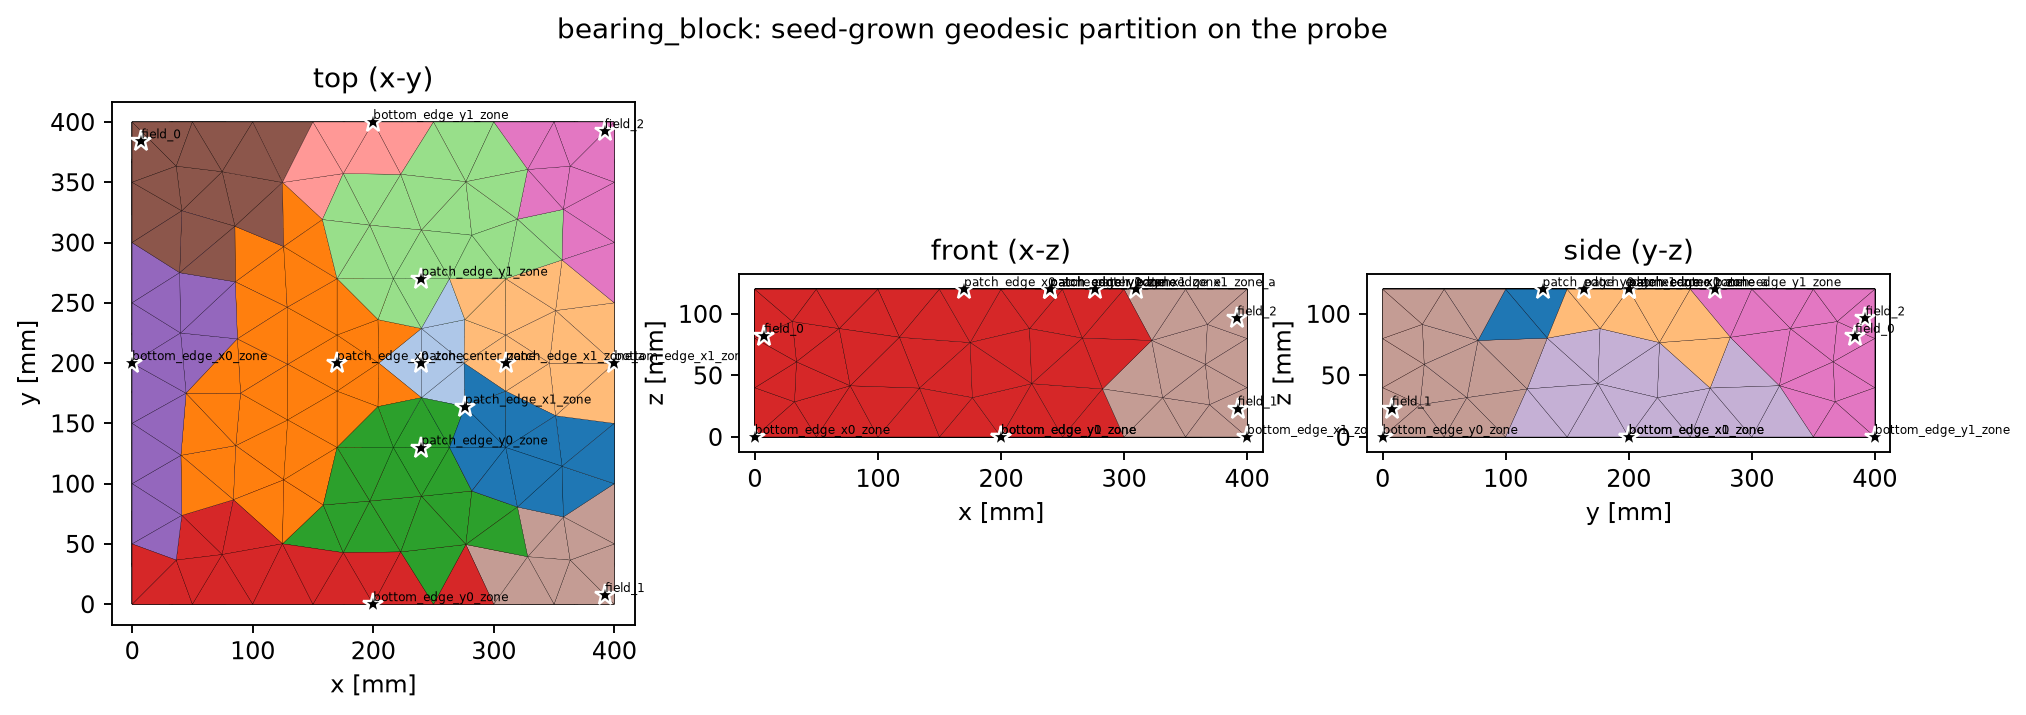
\includegraphics[width=\linewidth]{bearing_block_partition.png}
    \caption{Bearing block: seeds + geodesic regions.}
  \end{subfigure}\\[0.8em]
  \begin{subfigure}{\textwidth}
    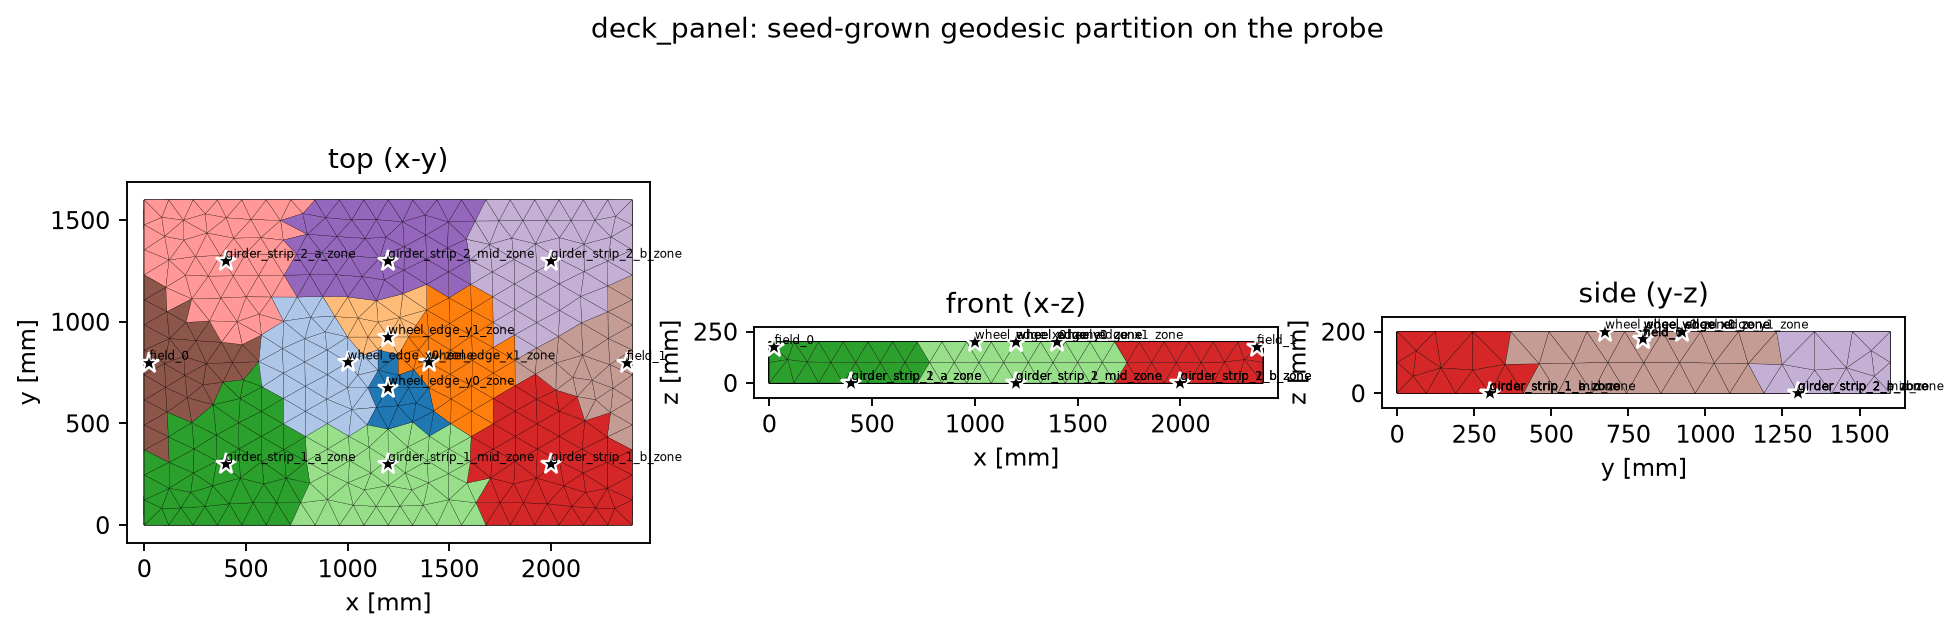
\includegraphics[width=\linewidth]{deck_panel_partition.png}
    \caption{Deck panel: seeds + geodesic regions.}
  \end{subfigure}
  \caption{[Pilot evidence for manuscript Fig.~2] Vision-seeded geodesic partitions on
  the two 3D bridge components (three orthographic views each; colours = regions,
  markers = named seeds). Source: \texttt{docs/evidence/}.}
  \label{fig:partitions}
\end{figure}

\begin{figure}[p]
  \centering
  \begin{subfigure}{0.49\textwidth}
    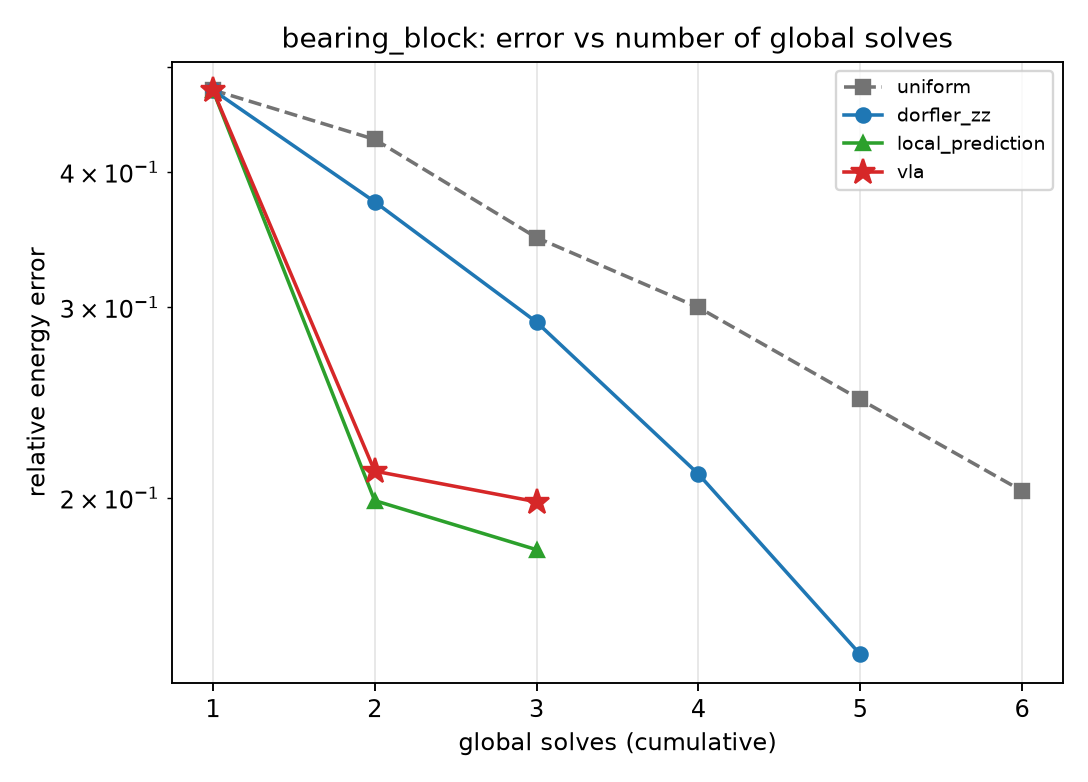
\includegraphics[width=\linewidth]{bearing_block_fig_error_vs_solves.png}
    \caption{Bearing block.}
  \end{subfigure}\hfill
  \begin{subfigure}{0.49\textwidth}
    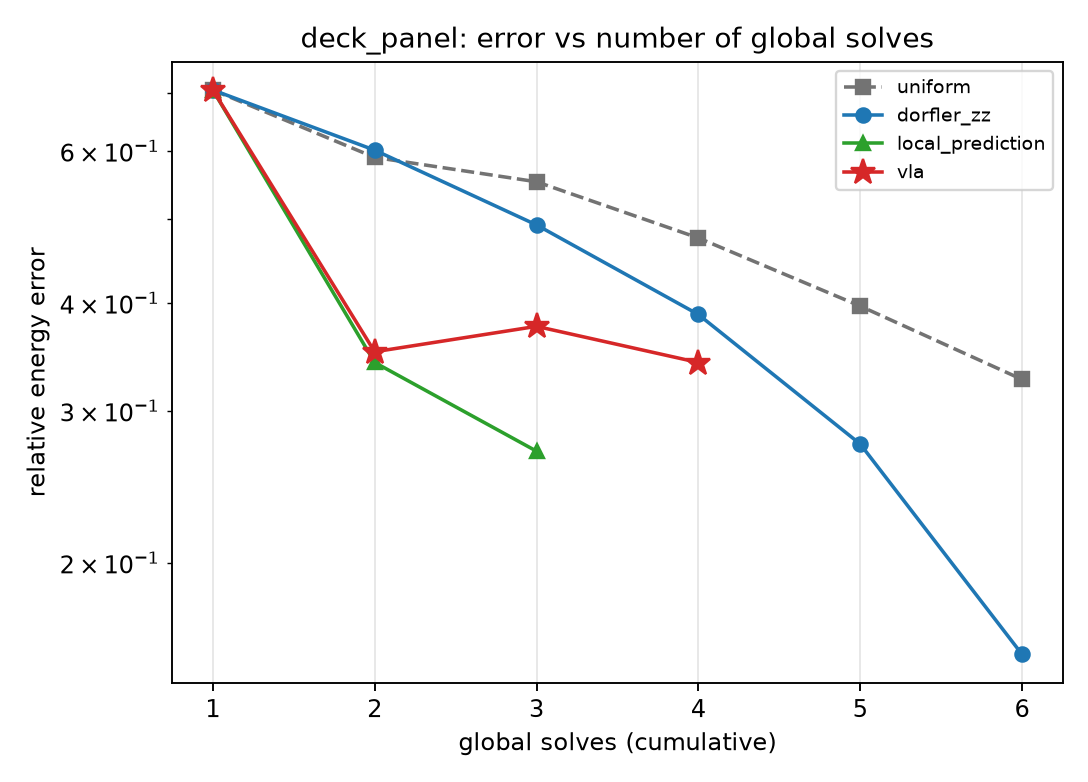
\includegraphics[width=\linewidth]{deck_panel_fig_error_vs_solves.png}
    \caption{Deck panel.}
  \end{subfigure}\\[0.6em]
  \begin{subfigure}{0.49\textwidth}
    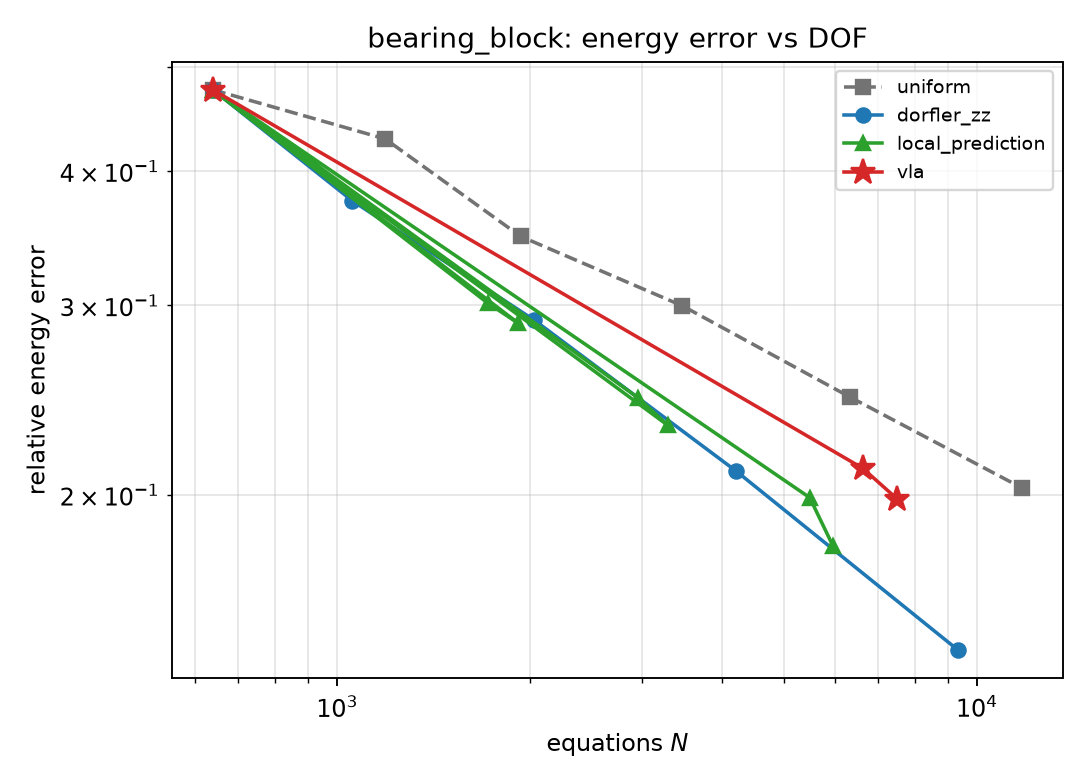
\includegraphics[width=\linewidth]{bearing_block_fig_error_vs_N.png}
    \caption{Bearing block, error vs $\Neq$.}
  \end{subfigure}\hfill
  \begin{subfigure}{0.49\textwidth}
    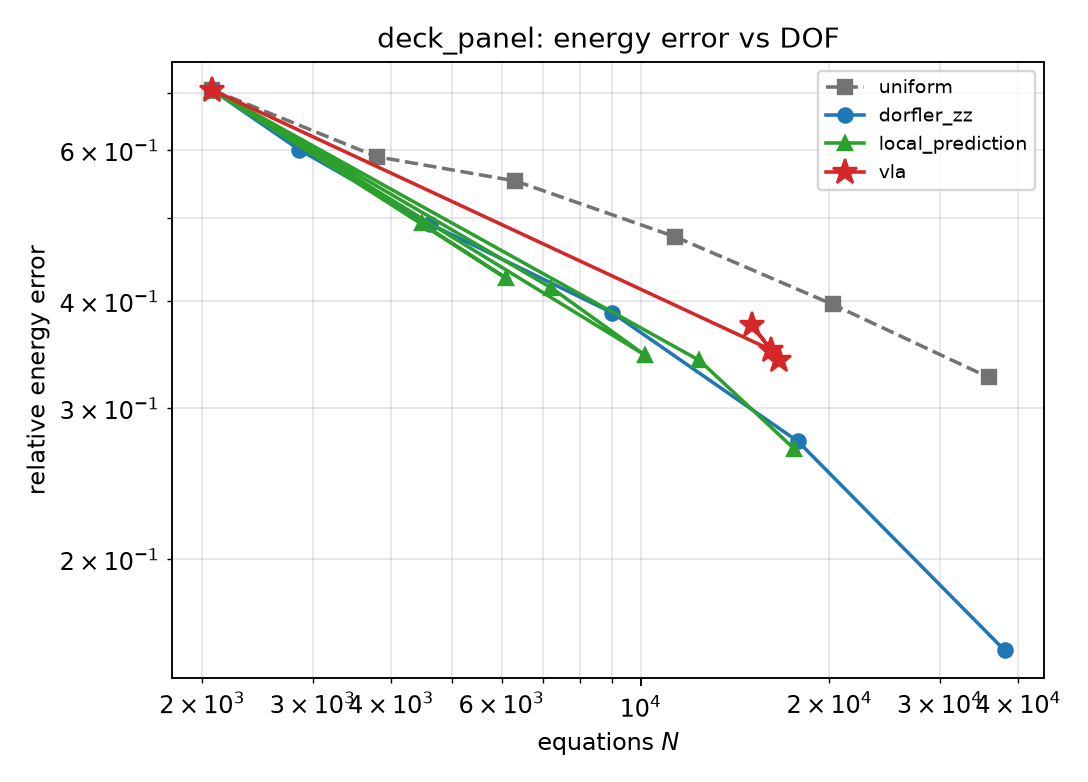
\includegraphics[width=\linewidth]{deck_panel_fig_error_vs_N.png}
    \caption{Deck panel, error vs $\Neq$.}
  \end{subfigure}
  \caption{[Pilot evidence for manuscript Figs.~4--5] Top: main axis A2$'$, energy
  error after the $k$-th global solve. Bottom: axis A1, error--$\Neq$ log--log with
  differing refinement atoms annotated; the D\"orfler crossover is exhibited, not
  hidden. Source: \texttt{docs/evidence/}.}
  \label{fig:curves}
\end{figure}

\section{Discussion}\label{sec:disc}
\begin{plan}
  \item Verdict subsection per pre-registered hypothesis:
        H1 (few-solve superiority, $k\in\{2,3,4\}$ + speed-up $\ge$1.5$\times$),
        H2 (hard-cap semantics: delivered $\Neq\in[90\%,105\%]$ of cap for VLA vs
        uncertified deviations $\ge$20\% for one-step prediction),
        H3 (training-free parity with learned baselines; total-cost accounting),
        H4 (crossover $k^*$ stated: pilot $\approx$5).
  \item Honesty boundaries (verbatim commitments): D\"orfler overtakes for
        $k\ge k^*$; local prediction wins some $k$ points on raw energy error while
        violating budget discipline (uncertified, $-26\%$/$+59\%$); 3D RL and
        supervised results are demo-scale and labelled as such.
  \item Why the mechanism works (tie each gain to an ablation): measured exponents
        kill the oscillation root cause; regional aggregation denoises pre-asymptotic
        indicators; drift feedback + projection make the cap a structural invariant
        rather than a hope; anchors inject drawing knowledge invisible to
        field-only indicators.
  \item Cost realism: PSO consumes surrogate evaluations only; LLM head latency and
        fallback rate; wall-clock per solve (1--20\,s on the pilot 4-core VM).
\end{plan}

\section{Limitations and future work}\label{sec:limits}
\begin{plan}
  \item Linear elasticity, C3D4 locking bias (same element family for all methods, so
        rankings remain meaningful; noted with G3 reference validation), single
        indicator (ZZ), one size per region, scripted head as vision-quality lower
        bound, LLM reproducibility handled by strict JSON + fallback reporting.
  \item Extension card (explicitly out of scope): contact/friction bearings, moving
        wheel-load envelopes, C3D10 verification, real bridge-drawing views for the
        LLM head, goal-oriented (dual-weighted) indicators.
\end{plan}

\section{Conclusions}\label{sec:concl}
\begin{plan}
  \item One-paragraph restatement of the narrow claim with final campaign numbers.
  \item The engineering message: a certified, training-free, few-solve regional loop
        formalising what analysts already do --- with the classical loop's asymptotic
        superiority explicitly conceded and located ($k^*$).
\end{plan}

% =====================================================================
\section*{CRediT authorship contribution statement}\label{sec:credit}
Author 1: Conceptualization, Methodology, Software, Investigation, Writing -- original
draft. Author 2: Validation, Writing -- review \& editing, Supervision. \todo{finalise}

\section*{Declaration of competing interest}
The authors declare no known competing financial interests or personal relationships.

\section*{Data availability}\label{sec:data}
All code, locked seeds, benchmark scripts and evidence figures are in the public
repository (\texttt{visionamr/}, \texttt{scripts/}, \texttt{docs/evidence/});
raw \texttt{.frd} ledgers of the full campaign will be archived (Zenodo DOI)
on acceptance. Reproduction entry points:
\texttt{scripts/run\_benchmark.py --problem bearing\_block --n-eq-budget 8000},
\texttt{scripts/run\_benchmark.py --problem deck\_panel --n-eq-budget 20000},
\texttt{scripts/make\_figures.py}, gate check \texttt{scripts/run\_smoke.py}.

\section*{Acknowledgements}
\todo{Funding and acknowledgements placeholder.}

% =====================================================================
\appendix
\section{Locked parameters (manuscript Appendix A)}
\begin{plan}
  \item VLA: gradation $g=0.9$; exponent clip $[0.6,4.5]$; PSO seed 17, position bound
        $0.8\to0.45$ (round $\ge$3); projection safety 0.97 / final 0.85; drift clip
        $[1.0,1.4]$; in-place certification gate 88\%/15\%; splits $\le$2 per round,
        $\le$14 regions; accuracy limit $=0.25\times$ probe indicator sum.
  \item Local prediction: exponent $(d+2)/2$; ratio clip $[1/6,1.8]$.
  \item DQN: 8-dim region features, 2-layer GCN, Double DQN, reward
        $10\,\Delta\log\sqrt{\Sigma\eta^2}-0.15$/step, over-budget $-2$ terminal, stop
        reward $2(\Neq/\text{cap})-1$.
  \item Supervised: 9-dim nodal features, MLP $64\times64$, target $\log(h/h_0)$.
  \item Full table generated from \texttt{locked.json} at campaign start (step S0).
\end{plan}

\section{Reproducibility and audit map (manuscript Appendix B)}
\begin{plan}
  \item Repository layout table (mirrors README): \texttt{visionamr/} core,
        \texttt{baselines/}, \texttt{vla/}, \texttt{scripts/}, \texttt{tests/}, CI
        workflow with G1 smoke gate.
  \item Baseline audit summary table from \texttt{docs/BASELINE\_AUDIT.md}
        (historical defect $\to$ fix $\to$ unit test).
  \item Campaign step cards S0--S9 with artefact names (no calendar claims).
\end{plan}

% =====================================================================
\begin{thebibliography}{00}
\small
\itemsep0.2em
% Representative skeleton; to be completed and verified before submission.
\bibitem{babuska78} I. Babu\v{s}ka, W.C. Rheinboldt, Error estimates for adaptive
finite element computations, SIAM J. Numer. Anal. 15 (1978) 736--754.
\bibitem{zz87} O.C. Zienkiewicz, J.Z. Zhu, A simple error estimator and adaptive
procedure for practical engineering analysis, Int. J. Numer. Methods Eng. 24 (1987)
337--357.
\bibitem{dorfler96} W. D\"orfler, A convergent adaptive algorithm for Poisson's
equation, SIAM J. Numer. Anal. 33 (1996) 1106--1124.
\bibitem{libettess95} X.D. Li, P. Bettess, Notes on mesh optimal criteria in adaptive
finite element computations, Commun. Numer. Methods Eng. 11 (1995) 911--915.
\bibitem{onate93} E. O\~nate, G. Bugeda, A study of mesh optimality criteria in
adaptive finite element analysis, Eng. Comput. 10 (1993) 307--321.
\bibitem{diez99} P. D\'iez, A. Huerta, A unified approach to remeshing strategies for
finite element $h$-adaptivity, Comput. Methods Appl. Mech. Eng. 176 (1999) 215--229.
\bibitem{yang23} J. Yang et al., Reinforcement learning for adaptive mesh refinement,
Proc. AISTATS (2023). \todo{verify}
\bibitem{foucart23} C. Foucart, A. Charous, P.F.J. Lermusiaux, Deep reinforcement
learning for adaptive mesh refinement, J. Comput. Phys. 491 (2023) 112381.
\bibitem{asmr23} N. Freymuth et al., Swarm reinforcement learning for adaptive mesh
refinement, Proc. NeurIPS (2023). \todo{verify}
\bibitem{meshingnet3d} Z. Zhang, P.K. Jimack, H. Wang, MeshingNet3D: efficient
generation of adapted tetrahedral meshes for computational mechanics, Adv. Eng.
Softw. 157--158 (2021) 103021. \todo{verify pages}
\bibitem{amber} AMBER: adaptive mesh generation by iterative mesh resolution
prediction. \todo{complete citation}
\bibitem{grefem} GReFEM: multimodal-LLM zero-shot identification of stress-critical
regions with one-shot budget allocation. \todo{complete citation}
\bibitem{feagpt} FeaGPT / VFEAgent: LLM agents for finite element workflows.
\todo{complete citation}
\bibitem{gmsh} C. Geuzaine, J.-F. Remacle, Gmsh: a 3-D finite element mesh generator
with built-in pre- and post-processing facilities, Int. J. Numer. Methods Eng. 79
(2009) 1309--1331.
\bibitem{ccx} G. Dhondt, The Finite Element Method for Three-Dimensional
Thermomechanical Applications, Wiley, 2004.
\bibitem{pso} J. Kennedy, R. Eberhart, Particle swarm optimization, Proc. IEEE Int.
Conf. Neural Networks (1995) 1942--1948.
\bibitem{ddqn} H. van Hasselt, A. Guez, D. Silver, Deep reinforcement learning with
double Q-learning, Proc. AAAI (2016) 2094--2100.
\bibitem{gcn} T.N. Kipf, M. Welling, Semi-supervised classification with graph
convolutional networks, Proc. ICLR (2017).
\end{thebibliography}

\end{document}
